%\documentclass[table]{article}
%\usepackage{beamerarticle}
\documentclass[10pt,xcolor=table,ignorenonframetext,aspectratio=169]{beamer}
%\documentclass[10pt,xcolor=table,ignorenonframetext]{beamer}
\mode<presentation>
{
  \usetheme{default}
  \useoutertheme{split}
% \usefonttheme{serif}
}

\usenavigationsymbolstemplate{}
\usepackage{amssymb}
\usepackage{amsmath}
\usepackage{setspace}
\usepackage{graphicx}
\usepackage{multirow}
\usepackage[english]{babel}
\usepackage[latin1]{inputenc}
\usepackage{bm}
\usepackage{graphicx}
\usepackage{multirow}
\usepackage{tikz}
\usepackage[english]{babel}
\usepackage[latin1]{inputenc}
%\usepackage{ulem}
\usepackage{pifont}
\usepackage{changepage}
%\usepackage{colortbl}
%\usepackage[table]{xcolor}
%\usepackage{xcolor}

\setbeamersize{text margin left=1cm,text margin right=5cm}

\setbeamertemplate{itemize item}[circle]
\setbeamertemplate{frametitle}[default][center]

\newlength{\wideitemsep}
\setlength{\wideitemsep}{\itemsep}
\addtolength{\wideitemsep}{4pt}
\let\olditem\item
\renewcommand{\item}{\setlength{\itemsep}{\wideitemsep}\olditem}

\newcommand{\HRule}{\rule{0.5\textwidth}{0.05mm}}

\usetikzlibrary{arrows,positioning,shapes}
\usetikzlibrary{decorations.pathreplacing}

\definecolor{blueish}{RGB}{97,156,255}
\definecolor{greenish}{RGB}{0,186,56}
\definecolor{reddish}{RGB}{248,118,109}

\definecolor{oiverm}{RGB}{213,94,0}
\definecolor{oiblue}{RGB}{0,114,178}
\definecolor{oigreen}{RGB}{0,158,115}
\definecolor{oipurple}{RGB}{204,121,167}
\definecolor{oiorange}{RGB}{230,159,0}
\definecolor{oisky}{RGB}{86,180,233}
\definecolor{oiyellow}{RGB}{240,228,66}
\definecolor{williams}{RGB}{81,38,152}

\definecolor{hue1}{RGB}{255,255,204}
\definecolor{hue2}{RGB}{161,218,180}
\definecolor{hue3}{RGB}{65,182,196}
\definecolor{hue4}{RGB}{44,127,184}
\definecolor{hue5}{RGB}{37,52,148}

\definecolor{dvg1}{RGB}{213,62,79}
\definecolor{dvg2}{RGB}{244,109,67}
\definecolor{dvg3}{RGB}{253,174,97}
\definecolor{dvg4}{RGB}{254,224,139}
\definecolor{dvg5}{RGB}{230,245,152}
\definecolor{dvg6}{RGB}{171,221,164}
\definecolor{dvg7}{RGB}{102,194,165}
\definecolor{dvg8}{RGB}{50,136,189}

\setbeamercolor{structure}{fg=williams,bg=williams!12}

\title{Impacts of Treatment-on-the-Treated, Slide \insertframenumber}
\subtitle{}

\author{Economics 379 (Professor Jakiela)}
\date{}



\begin{document}
	
	
	
%%%%%%%%%%%%%%%%%%%%%%%%%%%%%%%%%%%%%%%%%%%%%%%%%%%%%%%%%%%%%%%%%%%%%%%%%%
	% COURSE Title slide
%%%%%%%%%%%%%%%%%%%%%%%%%%%%%%%%%%%%%%%%%%%%%%%%%%%%%%%%%%%%%%%%%%%%%%%%%%
	
\begin{frame}<beamer:0>[plain]
	
	\begin{center}
		\begin{tikzpicture}
		
		\node [opacity=1] (bg)  {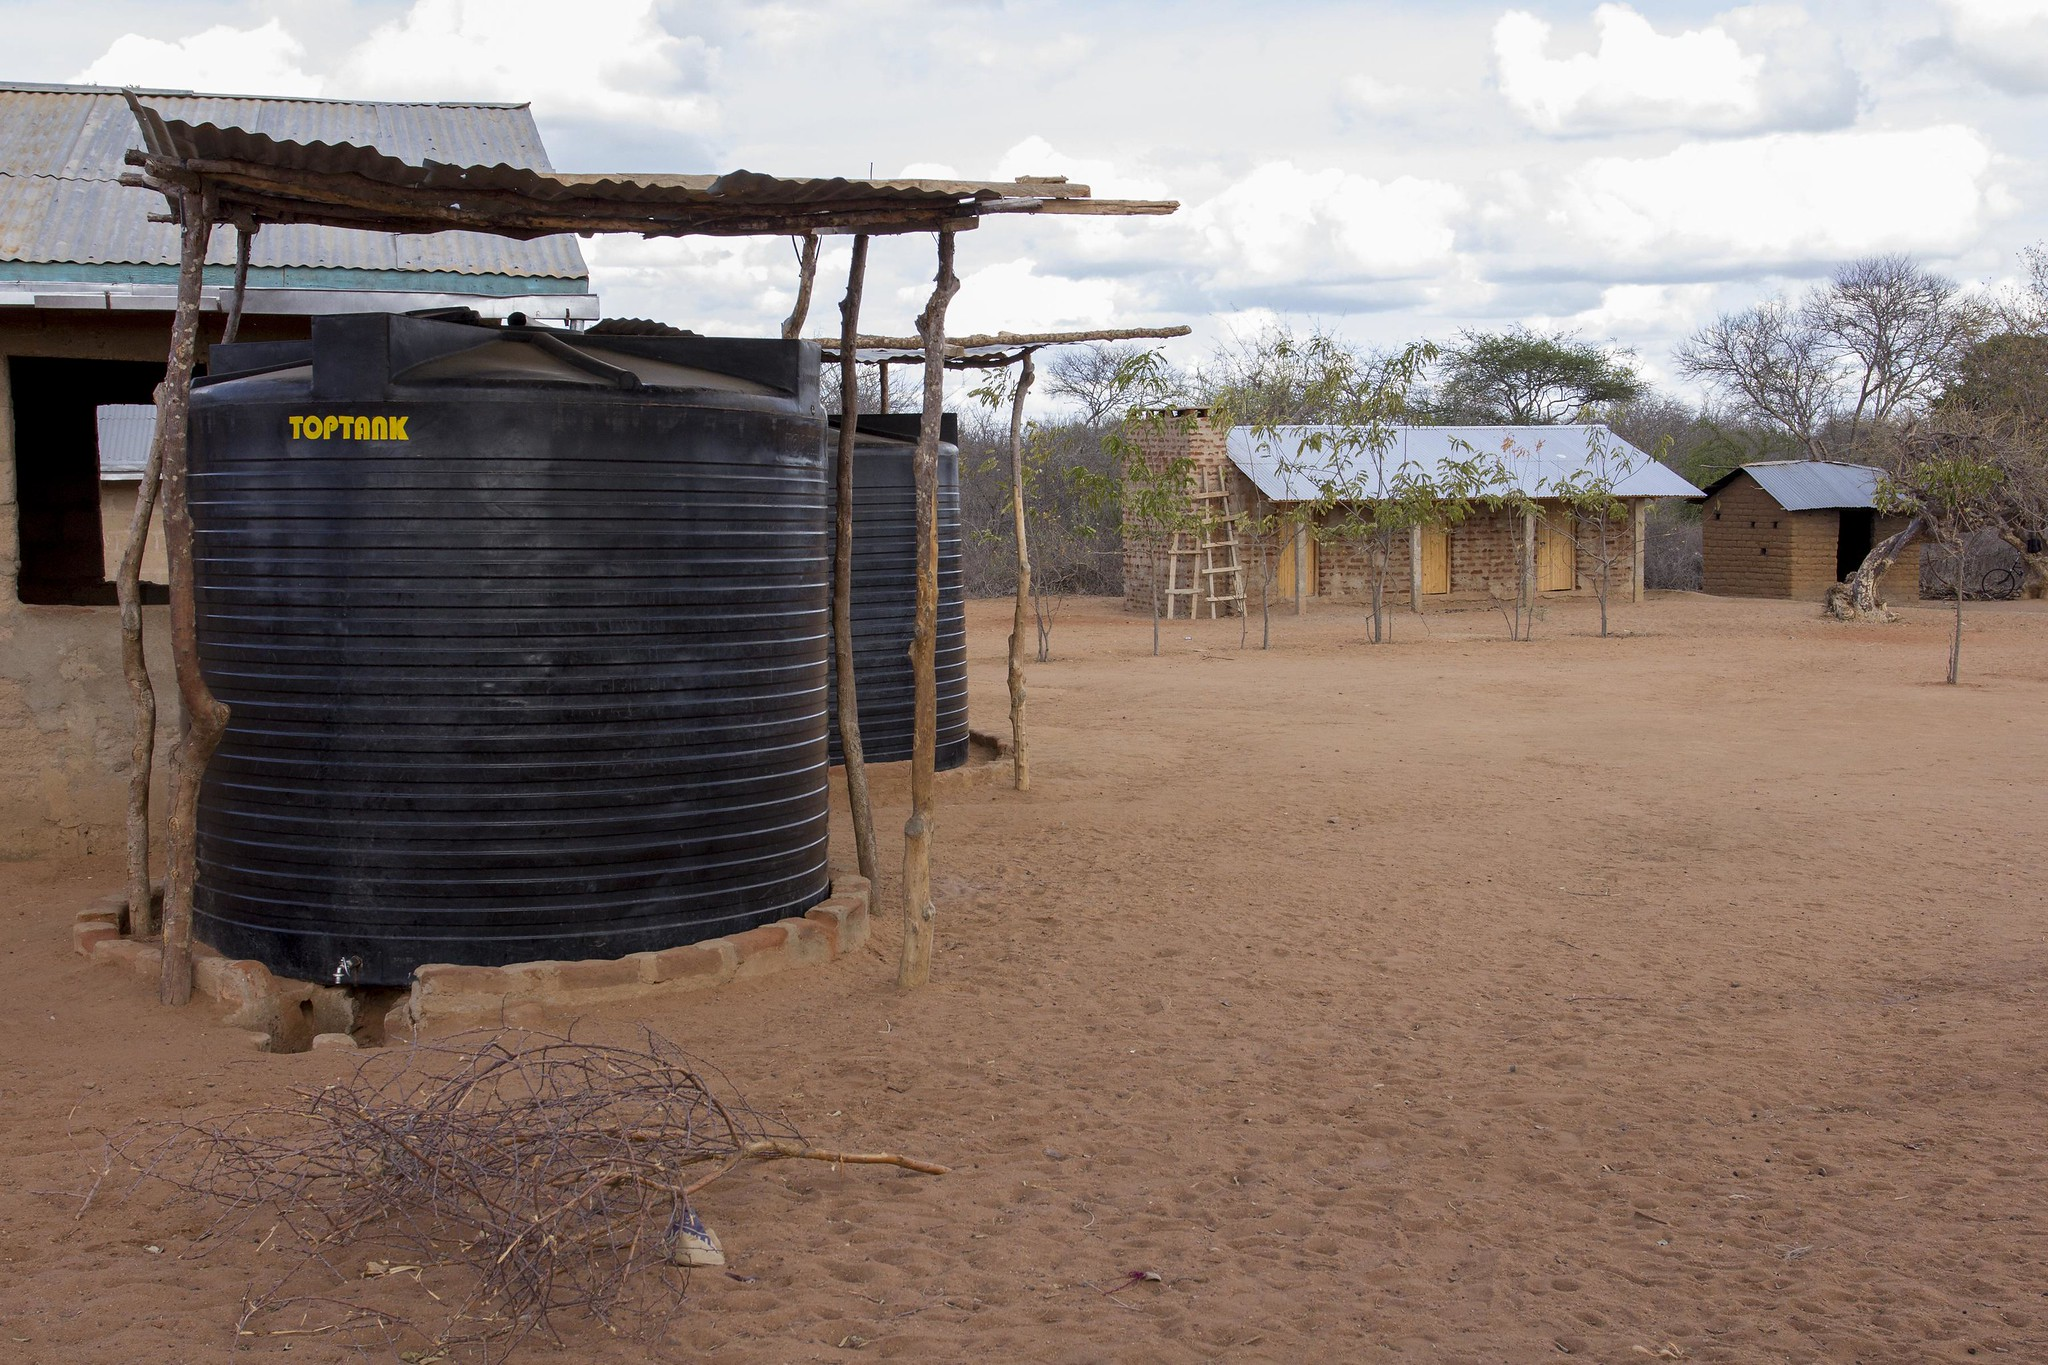
\includegraphics[keepaspectratio,height=0.9\paperheight]{photos/Kenya-cistern-Flore-de-Preneuf-2011-LARGE.jpg}};
		
		\node [anchor=east,align=right] at (6,-2.25) {\Large{\textcolor{white}{Williams College ECON 379:}}};		
		\node [anchor=east,align=right] at (6,-3) {\Large{\textcolor{white}{Program Evaluation for International Development}}};

		\node [anchor=east] at (6,-3.8) {\textcolor{yellow}{\tiny{photo:  Flore de Preneuf / World Bank}}};
		
		\end{tikzpicture}
	\end{center}
\end{frame}


%%%%%%%%%%%%%%%%%%%%%%%%%%%%%%%%%%%%%%%%%%%%%%%%%%%%%%%%%%%%%%%%%%%%%%%%%%
% LECTURE Title slide
%%%%%%%%%%%%%%%%%%%%%%%%%%%%%%%%%%%%%%%%%%%%%%%%%%%%%%%%%%%%%%%%%%%%%%%%%%

\begin{frame}[plain]

\only<beamer>{\begin{adjustwidth}{0cm}{-4cm}}

\begin{center}
	\begin{tikzpicture}
	
	\node [opacity=0.25] (bg)  {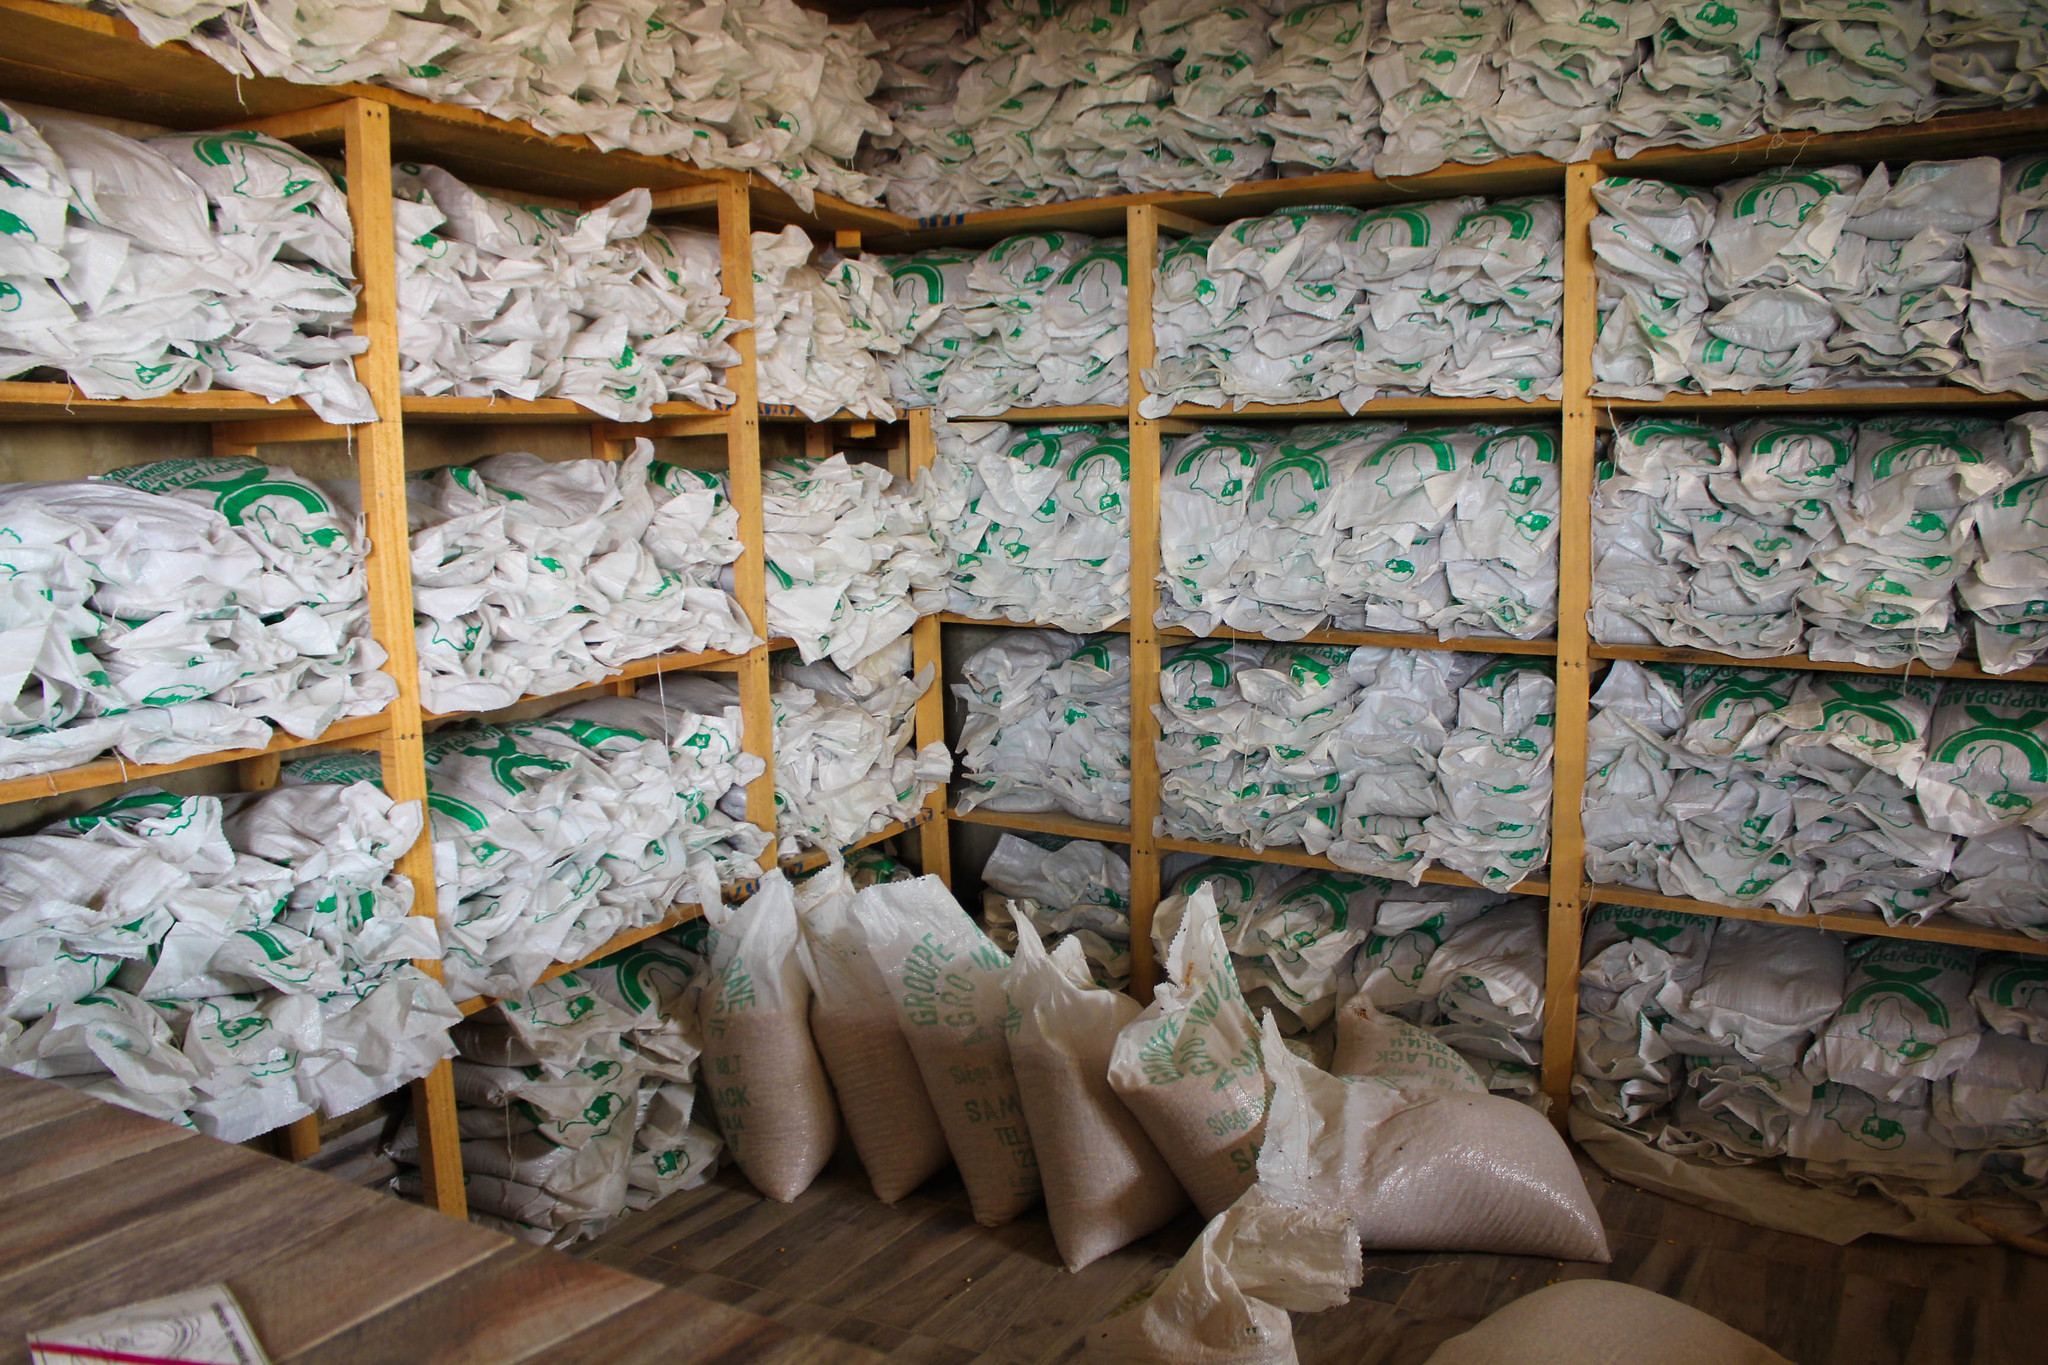
\includegraphics[keepaspectratio,height=0.9\paperheight]{photos/Senegal-WAAPP-seeds-Daniella-Van-Leggelo-Padilla-LARGE.jpg}};
	
	\node at (0,2.5) {\large{\textcolor{williams}{Williams College ECON 379:}}};		
	\node at (0,1.5) {\large{\textcolor{williams}{Program Evaluation for International Development}}};
	
	\node at (0,-0.5) {\large{\textcolor{williams}{\textbf{Module 8: Impacts of Treatment-on-the-Treated}}}};
	
	\node at (0,-2) {\large{\textcolor{williams}{Professor:  Pamela Jakiela}}};
	
	\node [anchor=east] at (6,-3.8) {\textcolor{yellow}{\tiny{photo:  Daniella Van Leggelo-Padilla / World Bank}}};
	
	\end{tikzpicture}
\end{center}
\only<beamer>{\end{adjustwidth}}
\end{frame}



%%%%%%%%%%%%%%%%%%%%%%%%%%%%%%%%%%%%%%%%%%%%%%%%%%%%%%%%%%%%%%%%%%%%%%%%%%%

%\begin{frame}<handout:0>[bg,plain]
\begin{frame}[plain]

\only<beamer>{\begin{adjustwidth}{0cm}{-4cm}}

\begin{center}
	
	%\Large{\textcolor{white}{Budget Sets and Budget Lines}}
	\Large{\textcolor{williams}{Imperfect Compliance}}
	
\end{center}

\only<beamer>{\end{adjustwidth}}
\end{frame}



%%%%%%%%%%%%%%%%%%%%%%%%%%%%%%%%%%%%%%%%%%%%%%%%%%%%%%%%%%%%%%%%%%%%%

\begin{frame}{How High Is Program Take-Up?}

\medskip
Even ``free'' programs costly for participants, take-up often low

%\medskip
\begin{center}
	\begin{small}
		\begingroup
		\setlength{\tabcolsep}{10pt} % Default value: 6pt
		\renewcommand{\arraystretch}{1.6} % Default value: 1
		\begin{tabular}{lll}
			\hline \hline
			\textbf{Intervention}	& \textbf{Take-Up}	& \textbf{Source} \\ \hline
			Business training		& 65\%				& McKenzie \& Woodruff (2013) \\
			Deworming medication	& 75\%				& Kremer \& Miguel (2007) \\
			Microfinance			& 13\% -- 31\%			& JPAL \& IPA (2015) \\
			\hline
		\end{tabular}	
		\endgroup
	\end{small}
\end{center}

\medskip
Only people who do a program can be impacted by the program$^{\ast}$

\medskip
\begin{itemize}
	
	\item[$\Rightarrow$] Might like to know how much program impacted participants \\
	(depending on our notion of treatment)
	
\end{itemize}

\medskip
\medskip
\medskip
\footnotesize{$^{\ast}$Some restrictions apply}

\end{frame}


%%%%%%%%%%%%%%%%%%%%%%%%%%%%%%%%%%%%%%%%%%%%%%%%%%%%%%%%%%%%%%%%%%%%%

\begin{frame}{A Thought Experiment}

\medskip
\begin{center}
	
	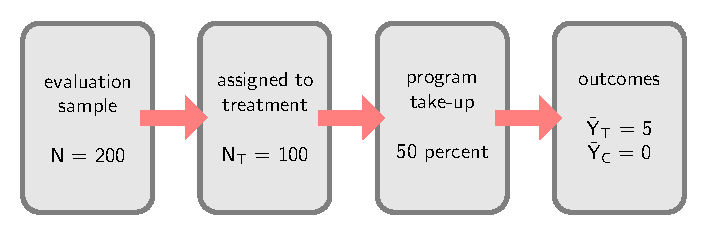
\includegraphics[trim = 0mm 0mm 0mm 0mm, clip, width=\textwidth]{tikz/pathway.pdf}
	
\end{center}

%\medskip
\medskip
Questions:  

\medskip
\begin{itemize}
	
	\item What was average outcome among those who did the program?
	
	\item What does this suggest about the impact of treatment?
	
\end{itemize}

\end{frame}



%%%%%%%%%%%%%%%%%%%%%%%%%%%%%%%%%%%%%%%%%%%%%%%%%%%%%%%%%%%%%%%%%%%%%

\begin{frame}{Imperfect Compliance}

\medskip
True model when outcomes impacted by program participation ($P_i$):

\begin{small}
	\begin{equation*}
	Y_i = \alpha + \beta \textcolor{red}{P_i} + \varepsilon_i
	\end{equation*}
\end{small}


\begin{itemize}
	
	\item Program take-up is endogenous conditional on treatment
	
	\item Only those assigned to treatment ($T_i = 1$) are eligible
	
	\item Not everyone participates:  $E [ P_i | T_i  = 1 ] = \lambda < 1$
	
\end{itemize}

\pause
\medskip
\medskip
What do we get from standard regression specification:
\begin{small}
	\begin{equation*}
	Y_i = \alpha + \beta \textcolor{red}{T_i} + \varepsilon_i
	\end{equation*}
\end{small}


\end{frame}


%%%%%%%%%%%%%%%%%%%%%%%%%%%%%%%%%%%%%%%%%%%%%%%%%%%%%%%%%%%%%%%%%%%%%

\begin{frame}{Imperfect Compliance}

\medskip
Modifying our standard OLS equation, we get:

\medskip
\begin{small}
	\begin{equation*}
	\begin{split}
	\hat{\beta} &= E \left[ Y_i \vert T_i = 1 \right] - E \left[ Y_i \vert T_i = 0 \right] \\
	& \\
	&= \alpha + \beta E \left[ P_i \vert T_i = 1 \right] + \varepsilon_i 
	- \left( \alpha + \beta  E \left[ P_i \vert T_i = 0 \right] + \varepsilon_i  \right) \\
	& \\
	&= \beta E \left[ P_i \vert T_i = 1 \right]  \\
	& \\
	&= \beta \lambda  \\
	\end{split}
	\end{equation*}
\end{small}

where $\lambda<1$ is the take-up rate in the treatment group

\medskip
\medskip
\structure{$\Rightarrow$ Low compliance scales down the estimated treatment effect}

\end{frame}


%%%%%%%%%%%%%%%%%%%%%%%%%%%%%%%%%%%%%%%%%%%%%%%%%%%%%%%%%%%%%%%%%%%%%%%

\begin{frame}{The Impact of Treatment on the Treated}

\begin{center}
	\begin{tikzpicture}
	
	% blank canvas
	\only<handout>{\fill[fill=white,draw=white,ultra thin]
	(0,0) -- (11,0) -- (11,6) -- (0,6) -- cycle;}
	\only<beamer>{\fill[fill=white,draw=white,ultra thin]
	(0,0) -- (14,0) -- (14,6) -- (0,6) -- cycle;}
	%\only<beamer>{\draw[draw=oiblue!60,fill=oiblue!10,opacity=0.5] (11,1) rectangle (14,5);}
	%\draw[step=1.0,gray!20,thin] (0,0) grid (11,6);
	
	%\pgfmathsetmacro\xshift{0.5cm};
	%\pgfmathsetmacro\yshift{5.5cm};
	
	\node[anchor=north,align=center,font=\small] (eq1) at (5,5.5) {$=$};
	\node[anchor=base east,align=right,font=\small] (eq1A) at (eq1.base west) {ATE};
	\node[anchor=base west,align=left,font=\small] (eq1Z) at (eq1.base east) {$\beta$};
	\node[anchor=base west,align=left,font=\small] (eq1Y) at ([xshift=-0.25cm]eq1Z.base east) {$\lambda$};
	
	\end{tikzpicture}
\end{center}
\end{frame}


%%%%%%%%%%%%%%%%%%%%%%%%%%%%%%%%%%%%%%%%%%%%%%%%%%%%%%%%%%%%%%%%%%%%%%%

\begin{frame}<handout:0>{The Impact of Treatment on the Treated}

\begin{center}
	\begin{tikzpicture}
	
	% blank canvas
	\only<handout>{\fill[fill=white,draw=white,ultra thin]
		(0,0) -- (11,0) -- (11,6) -- (0,6) -- cycle;}
	\only<beamer>{\fill[fill=white,draw=white,ultra thin]
		(0,0) -- (14,0) -- (14,6) -- (0,6) -- cycle;}
	%\only<beamer>{\draw[draw=oiblue!60,fill=oiblue!10,opacity=0.5] (11,1) rectangle (14,5);}
	%\draw[step=1.0,gray!20,thin] (0,0) grid (11,6);
	
	%\pgfmathsetmacro\xshift{0.5cm};
	%\pgfmathsetmacro\yshift{5.5cm};
	
	\node[anchor=north,align=center,font=\small] (eq1) at (5,5.5) {$=$};
	\node[red,anchor=base east,align=right,font=\small] (eq1A) at (eq1.base west) {ATE};
	\node[anchor=base west,align=left,font=\small] (eq1Z) at (eq1.base east) {$\beta$};
	\node[anchor=base west,align=left,font=\small] (eq1Y) at ([xshift=-0.25cm]eq1Z.base east) {$\lambda$};
	
	\node[red,anchor=north,align=center,font=\small] (lbl) at ([yshift=-1.25cm]eq1A.south) {average treatment effect};
	\node[red,anchor=north,align=center,font=\small] (lbl2) at (lbl.south) {(across entire treatment group)};
	\draw[red,->] (lbl.north) -- (eq1A.south);
	
	\end{tikzpicture}
\end{center}
\end{frame}



%%%%%%%%%%%%%%%%%%%%%%%%%%%%%%%%%%%%%%%%%%%%%%%%%%%%%%%%%%%%%%%%%%%%%%%

\begin{frame}<handout:0>{The Impact of Treatment on the Treated}

\begin{center}
	\begin{tikzpicture}
	
	% blank canvas
	\only<handout>{\fill[fill=white,draw=white,ultra thin]
		(0,0) -- (11,0) -- (11,6) -- (0,6) -- cycle;}
	\only<beamer>{\fill[fill=white,draw=white,ultra thin]
		(0,0) -- (14,0) -- (14,6) -- (0,6) -- cycle;}
	%\only<beamer>{\draw[draw=oiblue!60,fill=oiblue!10,opacity=0.5] (11,1) rectangle (14,5);}
	%\draw[step=1.0,gray!20,thin] (0,0) grid (11,6);
	
	%\pgfmathsetmacro\xshift{0.5cm};
	%\pgfmathsetmacro\yshift{5.5cm};
	
	\node[anchor=north,align=center,font=\small] (eq1) at (5,5.5) {$=$};
	\node[anchor=base east,align=right,font=\small] (eq1A) at (eq1.base west) {ATE};
	\node[red,anchor=base west,align=left,font=\small] (eq1Z) at (eq1.base east) {$\beta$};
	\node[anchor=base west,align=left,font=\small] (eq1Y) at ([xshift=-0.25cm]eq1Z.base east) {$\lambda$};
	
	\node[red,anchor=north,align=center,font=\small] (lbl) at ([yshift=-1.25cm]eq1Z.south) {impact of treatment};
	\node[red,anchor=north,align=center,font=\small] (lbl2) at (lbl.south) {(on those who participate)};
	\draw[red,->] (lbl.north) -- (eq1Z.south);
	
	\end{tikzpicture}
\end{center}
\end{frame}


%%%%%%%%%%%%%%%%%%%%%%%%%%%%%%%%%%%%%%%%%%%%%%%%%%%%%%%%%%%%%%%%%%%%%%%

\begin{frame}<handout:0>{The Impact of Treatment on the Treated}

\begin{center}
	\begin{tikzpicture}
	
	% blank canvas
	\only<handout>{\fill[fill=white,draw=white,ultra thin]
		(0,0) -- (11,0) -- (11,6) -- (0,6) -- cycle;}
	\only<beamer>{\fill[fill=white,draw=white,ultra thin]
		(0,0) -- (14,0) -- (14,6) -- (0,6) -- cycle;}
	%\only<beamer>{\draw[draw=oiblue!60,fill=oiblue!10,opacity=0.5] (11,1) rectangle (14,5);}
	%\draw[step=1.0,gray!20,thin] (0,0) grid (11,6);
	
	%\pgfmathsetmacro\xshift{0.5cm};
	%\pgfmathsetmacro\yshift{5.5cm};
	
	\node[anchor=north,align=center,font=\small] (eq1) at (5,5.5) {$=$};
	\node[anchor=base east,align=right,font=\small] (eq1A) at (eq1.base west) {ATE};
	\node[anchor=base west,align=left,font=\small] (eq1Z) at (eq1.base east) {$\beta$};
	\node[red,anchor=base west,align=left,font=\small] (eq1Y) at ([xshift=-0.25cm]eq1Z.base east) {$\lambda$};
	
	\node[red,anchor=north,align=center,font=\small] (lbl) at ([yshift=-1.25cm]eq1Y.south) {take-up rate};
	\node[red,anchor=north,align=center,font=\small] (lbl2) at (lbl.south) {(among those assigned to treatment)};
	\draw[red,->] (lbl.north) -- (eq1Y.south);
	
	\end{tikzpicture}
\end{center}
\end{frame}


%%%%%%%%%%%%%%%%%%%%%%%%%%%%%%%%%%%%%%%%%%%%%%%%%%%%%%%%%%%%%%%%%%%%%%%

\begin{frame}{The Impact of Treatment on the Treated}

\begin{center}
	\begin{tikzpicture}
	
	% blank canvas
	\only<handout>{\fill[fill=white,draw=white,ultra thin]
		(0,0) -- (11,0) -- (11,6) -- (0,6) -- cycle;}
	\only<beamer>{\fill[fill=white,draw=white,ultra thin]
		(0,0) -- (14,0) -- (14,6) -- (0,6) -- cycle;}
	%\only<beamer>{\draw[draw=oiblue!60,fill=oiblue!10,opacity=0.5] (11,1) rectangle (14,5);}
	%\draw[step=1.0,gray!20,thin] (0,0) grid (11,6);
	
	%\pgfmathsetmacro\xshift{0.5cm};
	%\pgfmathsetmacro\yshift{5.5cm};
	
	\node[anchor=north,align=center,font=\small] (eq1) at (5,5.5) {$=$};
	\node[anchor=base east,align=right,font=\small] (eq1A) at (eq1.base west) {ATE};
	\node[anchor=base west,align=left,font=\small] (eq1Z) at (eq1.base east) {$\beta$};
	\node[anchor=base west,align=left,font=\small] (eq1Y) at ([xshift=-0.25cm]eq1Z.base east) {$\lambda$};

	\node[anchor=base,align=center,font=\small] (eq2) at ([yshift=-0.625cm]eq1.base) {$=$};
	\node[red,anchor=base east,align=right,font=\small] (eq2A) at (eq2.base west) {$\beta$};
	\node[anchor=base west,align=left,font=\small] (eq2Z) at (eq2.base east) {ATE/$\lambda$};
	
	\node[red,anchor=north,align=center,font=\small] (lbl) at ([yshift=-1.25cm]eq2A.south) {impact of treatment on the treated};
	\draw[red,->] (lbl.north) -- (eq2A.south);

	
	\end{tikzpicture}
\end{center}
\end{frame}




%%%%%%%%%%%%%%%%%%%%%%%%%%%%%%%%%%%%%%%%%%%%%%%%%%%%%%%%%%%%%%%%%%%%%

\begin{frame}{Treatment on the Treated:  Intuition}

\medskip
The \textbf{treatment on the treated (TOT)} estimator:

\medskip
\begin{small}
	\begin{equation*}
	\hat{\beta}_{tot} = \frac{E \left[ Y_i \vert T_i = 1 \right] - E \left[ Y_i \vert T_i = 0 \right]}{ 
		E \left[ P_i \vert T_i = 1 \right] - E \left[ P_i \vert T_i = 0 \right]}
	\end{equation*}
\end{small}

\medskip
TOT scales up ITT effect to reflect imperfect take-up

\medskip
\begin{itemize}
	
	\item Assumption:  treatment only works through program take-up
	
	\medskip
	\begin{itemize}
		
		\item Not always obvious whether this is true
		
	\end{itemize}
	
\end{itemize}

\end{frame}




%%%%%%%%%%%%%%%%%%%%%%%%%%%%%%%%%%%%%%%%%%%%%%%%%%%%%%%%%%%%%%%%%%%%%

\begin{frame}{Treatment on the Treated:  Implementation}

\medskip
\textbf{Two regressions:}

\medskip
Impact of assignment to treatment on outcome of interest:
\begin{small}
	\begin{equation*}
	Y_i = \alpha_2 + \beta_1 T_i + \nu_i \ \ \ \ [\textsf{intent-to-treat}]
	\end{equation*}
\end{small}

%\medskip
Impact of assignment to treatment on program participation:
\begin{small}
	\begin{equation*}
	P_i = \alpha_2 + \beta_2 T_i + \nu_i \ \ \ \ [\textsf{first stage}]
	\end{equation*}
\end{small}

\pause
\textcolor{red}{Impact of treatment on the treated:  $\beta_{tot} = \beta_{itt} / \beta_{fs}$}


\end{frame}


%%%%%%%%%%%%%%%%%%%%%%%%%%%%%%%%%%%%%%%%%%%%%%%%%%%%%%%%%%%%%%%%%%%%%

\begin{frame}{Treatment on the Treated:  Implementation}

\medskip
Estimated via two-stage least squares (2SLS):
\begin{small}
	\begin{equation*}
	\begin{split}
	Y_i &= \alpha_1 + \beta_{IV} \hat{P}_i + \varepsilon_i \ \ \ \ [\textsf{IV regression}] \\
	& \\
	P_i &= \alpha_2 + \beta_2 T_i + \nu_i \ \ \ \ [\textsf{first stage}]\\
	\end{split}
	\end{equation*}
\end{small}


\medskip
Easy to implement using Stata's \textcolor{red}{\texttt{ivregress 2sls}} command 

\medskip
\begin{itemize}
	
	\item Running two (separate) regressions yields wrong standard error
	
\end{itemize}

\end{frame}


%%%%%%%%%%%%%%%%%%%%%%%%%%%%%%%%%%%%%%%%%%%%%%%%%%%%%%%%%%%%%%%%%%%%%

\begin{frame}{Treatment on the Treated:  Implementation}

\medskip
\begin{center}
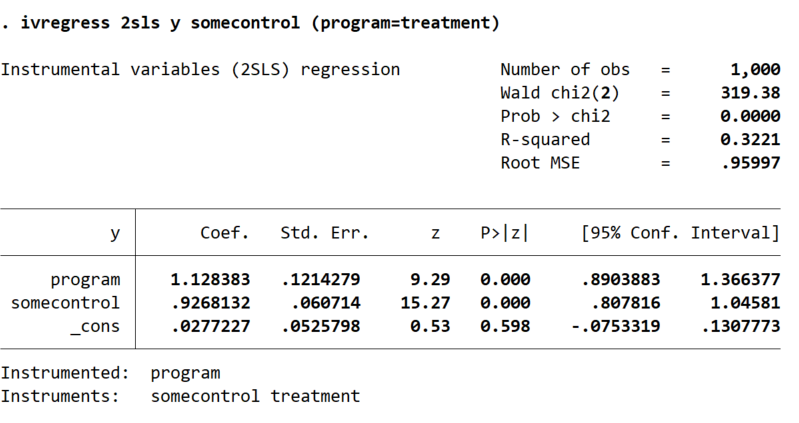
\includegraphics[width=\textwidth]{img/StataIV1.png}
\end{center}

\end{frame}


%%%%%%%%%%%%%%%%%%%%%%%%%%%%%%%%%%%%%%%%%%%%%%%%%%%%%%%%%%%%%%%%%%%%%

\begin{frame}{Treatment on the Treated:  Implementation}

\medskip
\begin{center}
	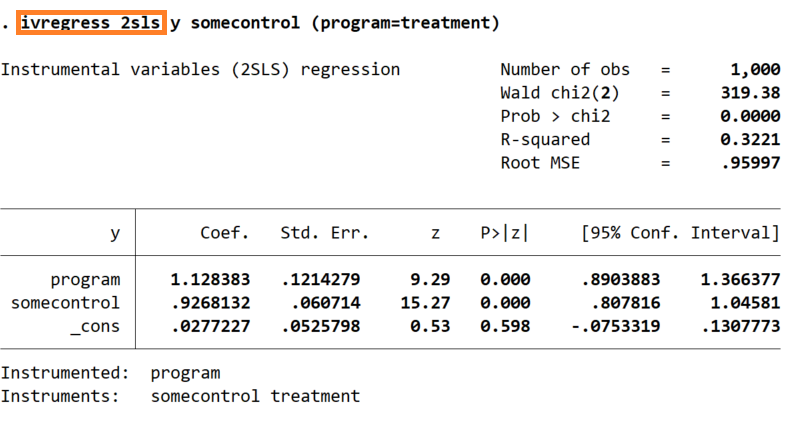
\includegraphics[width=\textwidth]{img/StataIV1a.png}
\end{center}

\end{frame}


%%%%%%%%%%%%%%%%%%%%%%%%%%%%%%%%%%%%%%%%%%%%%%%%%%%%%%%%%%%%%%%%%%%%%

\begin{frame}{Treatment on the Treated:  Implementation}

\medskip
\begin{center}
	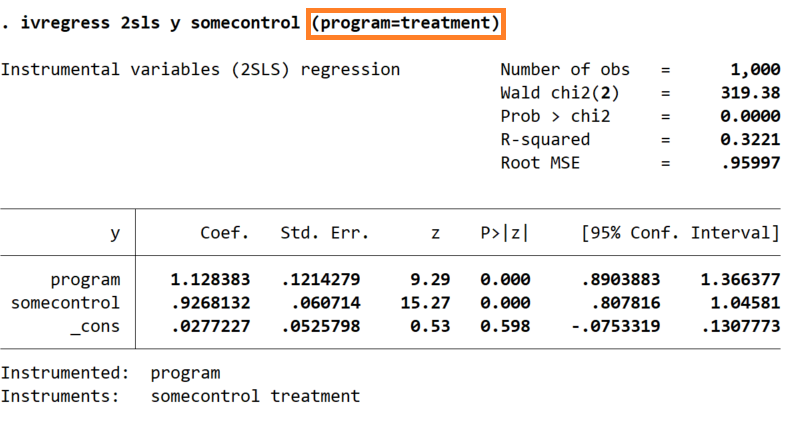
\includegraphics[width=\textwidth]{img/StataIV1b.png}
\end{center}

\end{frame}


%%%%%%%%%%%%%%%%%%%%%%%%%%%%%%%%%%%%%%%%%%%%%%%%%%%%%%%%%%%%%%%%%%%%%

\begin{frame}{Treatment on the Treated:  Implementation}

\medskip
\begin{center}
	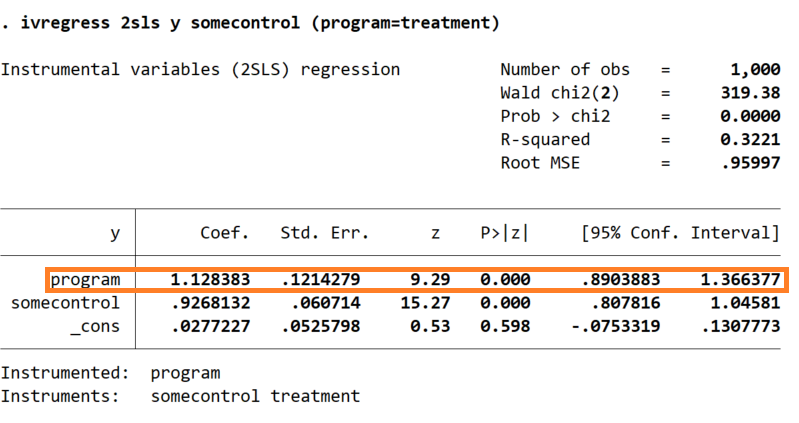
\includegraphics[width=\textwidth]{img/StataIV2.png}
\end{center}

\end{frame}



%%%%%%%%%%%%%%%%%%%%%%%%%%%%%%%%%%%%%%%%%%%%%%%%%%%%%%%%%%%%%%%%%%%%%

\begin{frame}{Assumptions Required for IV Estimation of TOT Effect}

\medskip
\begin{enumerate}
	
	\item Instrument is exogenous (OK in an RCT)
	
	\item Instrument is correlated with treatment (first stage)
	
	\item Only impacts outcomes through take-up (exclusion restriction)
	
	\item Monotonicity (optional requirement)
	
	\medskip
	\begin{itemize}
		
		\item Not required if treatment effects are homogeneous
		
	\end{itemize}
	
\end{enumerate}


\end{frame}




%%%%%%%%%%%%%%%%%%%%%%%%%%%%%%%%%%%%%%%%%%%%%%%%%%%%%%%%%%%%%%%%%%%%%

\begin{frame}{What Does Treatment on the Treated Measure?}

\medskip
\begin{center}
	\begin{small}
		\begingroup
		\setlength{\tabcolsep}{10pt} % Default value: 6pt
		\renewcommand{\arraystretch}{2} % Default value: 1
		\begin{tabular}{ccc}
			$T = 0$	& & $T = 1$ \\ \cline{1-1} \cline{3-3} 
			& & \\ [-5.4ex]
			\cellcolor{greenish!20}{always takers} & & \cellcolor{greenish!20}{always takers} \\ \cline{1-1}
			compliers		&	& \cellcolor{greenish!20}{compliers} \\  \cline{3-3} 
			never takers		&	& never takers  \\ \cline{1-1} \cline{3-3}
		\end{tabular}	
		\endgroup
	\end{small}
\end{center}

\medskip
\medskip
TOT estimates local average treatment effect (LATE) on \textbf{compliers}

\medskip
\begin{itemize}
	
	\item Monotonicity assumption:  there are no \textbf{defiers}
	
	\item We can't estimate impacts on \textbf{always takers} and \textbf{never takers} because their treatment status doesn't change take-up decision
	
\end{itemize}

\end{frame}









\end{document}